\documentclass[10pt]{article}
\usepackage{amsmath}
\usepackage{amssymb}
\usepackage{graphicx}
\usepackage{hyperref}
\usepackage{geometry}
\usepackage{titlesec}
\usepackage{tikz}
\usetikzlibrary{positioning,matrix,decorations.pathreplacing}
\geometry{a4paper, margin=1in}

\title{
    Response to He et al., (2016) \\
}
\author{Matthew Evans}
\date{\today}

\begin{document}

\maketitle

\section*{Overview}
% Articulate what problem or issue does the authors' work addresses or what they aimed to achieve using absolutely no technical jargon.
% Degradation problem
Adding layers to a network's architecture increases its complexity and potentially its predictive ability. Yet, beyond a certain layer depth, accuracy degrades. In \cite{7780459},  He et al. propose a novel approach to overcome this problem, unlocking the potential of deep networks (i.e., with hundreds of layers) for image classification tasks.


\section*{Approach}
% Understand and articulate how things were done prior to the innovation described in the paper.
% Residual connections

The layers of a network can be thought of as functions with the output of one function being the input of the next. The network as a whole can thus be viewed as the function composition
\[
    Y = H_n \circ H_{n-1}\circ H_{n-2} \circ \dots \circ H_{1}(x)
\]
with \(Y\) as the final output, \(H_1, H_2, \dots, H_{n}\) as the hidden layers, and \(x\) as the input.

Thus, the goal of training is to learn sufficiently close approximations of each layer's function so as to yield the correct final output. In some task domains, such as image classification, each of these functions can be thought of as extracting increasingly sophisticated features (e.g., edges, then textures, then objects) from the input data to aid in the classification task. Yet in networks with many layers, the optimal adjustment made by each layer may be small, or even no adjustment at all. In other words, if a object is already sufficient identifiable at the \(i\)th layer, there is no need to extract additional features in the remaining \(n-i\) layers. In fact, learning the remaining \(n-i\) functions is a waste of computation at best and, at worst, can be detrimental to the network's accuracy, an issue known as the \textit{degradation problem}. The authors introduce the strategy of using \textit{shortcut connections} to overcome the degradation problem.

\subsection*{Residual Functions and Shortcut Connections}
In \textit{plain networks} (i.e., those not using the strategies introduced in \cite{7780459}), for each hidden layer, the network aims to learn that layer's function,
\[
    H_i(x_{i}).
\]
As noted above, in deep architectures for image classification, difference between a layer's input and output is often small. That is,
\[
    H_i(x_{i}) = F(x_{i}) + x_{i}
\]
where \(F(x_{i-1})\) is a \textit{residual function} capturing this small difference between input and output. The authors' key insight is that since \(H_i(x_{i}) \approx x_{i}\), the network's attention should be focused on the more tractable problem of computing \(F(x_{i})\). To force this learning behavior, the authors' proposed \textit{residual network} architecture introduces a \textit{shortcut connection}, supplying a given layer's input as supplemental \textit{output} of a subsequent layer's activation function (Fig. \ref*{fig:residual}).


\subsection*{Additional Benefits}
The authors demonstrate the following benefits of this strategy.
\begin{itemize}
    \item Using shortcut layers does not introduce any additional parameters, and the introduction of the sum adds minimal computational overhead.
    \item Shortcut layers can be used with variety of layer types (e.g., fully connected, convolutional, etc.).
    \item Shortcut layers can be effectively added to existing network architectures, yielding faster convergence, and in the case of deeper networks, dramatically improve accuracy.
\end{itemize}


\begin{figure}[h]
    \centering
    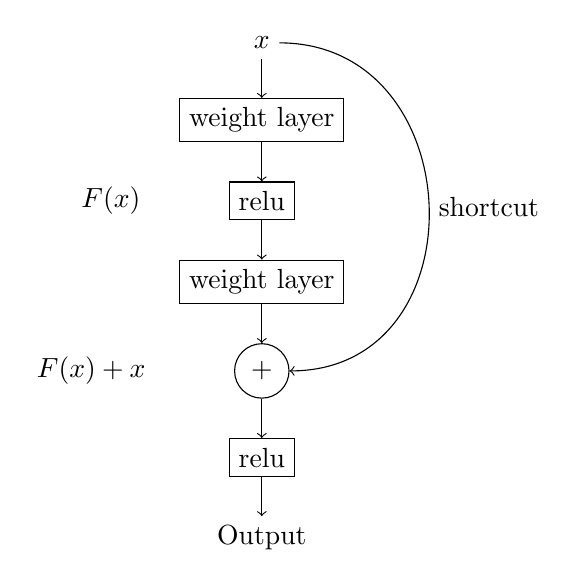
\begin{tikzpicture}[node distance=0.5cm]
        % Nodes
        \node (input) at (0, 0) {$x$};
        \node[draw, rectangle, below=of input] (layer1) {weight layer};
        \node[draw, rectangle, below=of layer1] (relu1) {relu};
        \node[draw, rectangle, below=of relu1] (layer2) {weight layer};
        \node[circle, draw, below=of layer2] (plus) {$+$};
        \node[draw, rectangle, below=of plus] (relu2) {relu};
        \node[below=of relu2] (output) {Output};

        % Shortcut connection
        \draw[->] (input.east) to[out=0, in=0, looseness=1.5] node[right] {shortcut} (plus.east);

        % Arrows
        \draw[->] (input) -- (layer1);
        \draw[->] (layer1) -- (relu1);
        \draw[->] (relu1) -- (layer2);
        \draw[->] (layer2) -- (plus);
        \draw[->] (plus) -- (relu2);
        \draw[->] (relu2) -- (output);

        % Text for F(x)
        \node[left=1cm of relu1] {$F(x)$};

        % Text for F(x) + x
        \node[left=1cm of plus] {$F(x) + x$};
    \end{tikzpicture}
    \caption{A residual learning building block as described by \cite{7780459}.}
    \label{fig:residual}
\end{figure}


% Plain networks (no residual connections)
% Fewer layers
% highway networks

% The "constructed" solution paradox and the degradation problem
% Why the degradation problem isn't due to over-fitting


% Understand and articulate what is novel about the author's approach, and what about it is particularly promising.

% Describe residual connections
% Empirical evidence shows that the changes between subsequent deep layers are small, thus it is easier to learn the delta than to learn the delta AND the original value.
% Particular relevance to image classification; describe how the different layers represent progressively enhanced features.
% Math of residual layers
% Diagram showing residual layers
% You can essentially "bolt it on" to previous existing network architecture; works fine with convolutional layers; doesn't add any additional parameters; if used with existing network (i.e., if you don't increase the number of layers over an existing architecture), it increases the speed of convergence. 

\section*{Measures of Success}
The authors validate their approach through experiments on the ImageNet 2012 dataset, showing that ResNets significantly outperform plain networks in both accuracy and convergence. For instance, a 34-layer ResNet achieves a top-1 error rate of 25.03\% compared to 28.54\% for a plain network, with even greater gains for deeper networks (e.g., 19.38\% for a 152-layer ResNet). ResNets are also shown to converge faster during training, easing optimization.

On the CIFAR-10 dataset, ResNets achieve state-of-the-art results with fewer parameters and faster convergence, further demonstrating their effectiveness in addressing the degradation problem and enabling the training of very deep networks.

\section*{Considerations}

\begin{itemize}
    \item While the authors offer conjecture for the exact root cause of the degradation problem, suggesting that perhaps deep plain networks suffer from exponentially low convergence rates, they offer no sure answer. While this doesn't detract from their demonstrated performance gains, it can't make sure claims on other problem domains.
    \item The authors suggest that their experiments with a variety of vision related tasks indicate that residual learning is a generic principle, and thus expect that it is applicable in non-vision problems, but offer no proof of this.
\end{itemize}

% Understand and articulate the risks and/or weaknesses of the author's approach.

% Unclear how this might work in other problem domains. Seems particularly well suited to image feature extraction.


% Understand and articulate the measures of success the authors used to validate their findings.

% their success in performance in competitions 


\section*{Impact}
% Understand and articulate the impact of the innovations described in the paper.

% Solves for the degradation problem and enables performance gains to continue scaling with network depths, providing a path forward for improved learning models. 

Since ResNet \cite{7780459}, residual functions and shortcut connections have been adopted in a variety of problem domains and deep network architectures including, but also well beyond that of image classification and object detection. Of particular note are \textit{transformer} network architectures which use a similar concept (``add \& norm'' layers). Popular examples include BERT with 12+ layers \cite{DBLP:journals/corr/abs-1810-04805}, and GPT-3 with 96 layers\cite{DBLP:journals/corr/abs-2005-14165}.

\bibliographystyle{unsrt}
\bibliography{references}

\end{document}